\documentclass{article}

% ------------------------------------------------
% Packages
% ------------------------------------------------
\usepackage{amsmath,amssymb,amsthm}
\usepackage{geometry}
\usepackage{array}
\usepackage{booktabs}
\usepackage{enumitem}
\usepackage{fancyhdr}
\usepackage{setspace}
\usepackage{tikz}
\usepackage{tikz-3dplot}
\usetikzlibrary{arrows.meta}

\geometry{
    margin=1in
}

\onehalfspacing

\pagestyle{fancy}
\fancyhf{}
\lhead{APM1220: Applied Multivariate Data Analysis}
\rhead{FA 2}
\cfoot{\thepage}

\begin{document}


% ================
% PROBLEM 3.1
% ================

\section*{Problem 3.1 -- Sample Geometry}

Given the data matrix

\[
X=
\begin{bmatrix}
9&1\\
5&3\\
1&2
\end{bmatrix}.
\]

Thus, the three observations are

\[
(9,1),\qquad (5,3),\qquad (1,2).
\]

The two variable vectors are

\[
\mathbf y_1=
\begin{bmatrix}
9\\5\\1
\end{bmatrix},
\qquad
\mathbf y_2=
\begin{bmatrix}
1\\3\\2
\end{bmatrix}.
\]

% --------------
% PART (a)
% ---------------

\subsection*{(a) Scatter plot in \(p=2\) dimensions}

The sample mean is

\[
\bar{x}_1
=
\frac{9+5+1}{3}
=5,
\]

and

\[
\bar{x}_2
=
\frac{1+3+2}{3}
=2.
\]

Therefore,

\[
\boxed{
\bar{\mathbf{x}}
=
\begin{bmatrix}
5\\
2
\end{bmatrix}}
\]

and the sample mean is the point

\[
\boxed{(5,2)}.
\]

The scatter plot is shown below.

\begin{center}
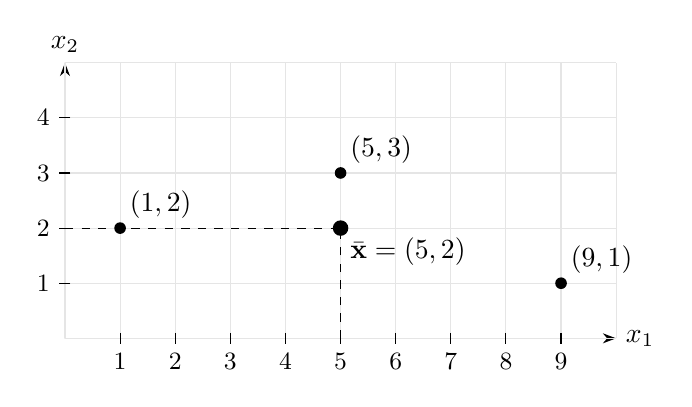
\begin{tikzpicture}[>=Stealth, scale=0.7]

    % Axes
    \draw[->] (0,0) -- (10,0) node[right] {$x_1$};
    \draw[->] (0,0) -- (0,5) node[above] {$x_2$};

    % Grid
    \draw[step=1cm,gray!20] (0,0) grid (10,5);

    % Tick labels x1
    \foreach \x in {1,...,9}
        \draw (\x,0.1) -- (\x,-0.1)
        node[below] {\small \x};

    % Tick labels x2
    \foreach \y in {1,...,4}
        \draw (0.1,\y) -- (-0.1,\y)
        node[left] {\small \y};

    % Data points
    \fill (9,1) circle (3pt)
        node[above right] {$(9,1)$};

    \fill (5,3) circle (3pt)
        node[above right] {$(5,3)$};

    \fill (1,2) circle (3pt)
        node[above right] {$(1,2)$};

    % Sample mean
    \fill (5,2) circle (4pt)
        node[below right] {$\bar{\mathbf{x}}=(5,2)$};

    % Dashed lines showing mean location
    \draw[dashed] (5,0) -- (5,2);
    \draw[dashed] (0,2) -- (5,2);

\end{tikzpicture}
\end{center}

% ------------
% PART (b)
% ------------

\subsection*{(b) \(n=3\)-dimensional representation}

The two variables can be represented as vectors in
\(\mathbb{R}^3\):

\[
\mathbf y_1=
\begin{bmatrix}
9\\5\\1
\end{bmatrix},
\qquad
\mathbf y_2=
\begin{bmatrix}
1\\3\\2
\end{bmatrix}.
\]

The sample means are

\[
\bar{x}_1=5,
\qquad
\bar{x}_2=2.
\]

Thus,

\[
\bar{x}_1\mathbf{1}
=
\begin{bmatrix}
5\\5\\5
\end{bmatrix},
\qquad
\bar{x}_2\mathbf{1}
=
\begin{bmatrix}
2\\2\\2
\end{bmatrix}.
\]

The deviation vectors are

\[
\mathbf y_1-\bar{x}_1\mathbf{1}
=
\begin{bmatrix}
9\\5\\1
\end{bmatrix}
-
\begin{bmatrix}
5\\5\\5
\end{bmatrix}
=
\boxed{
\begin{bmatrix}
4\\0\\-4
\end{bmatrix}},
\]

and

\[
\mathbf y_2-\bar{x}_2\mathbf{1}
=
\begin{bmatrix}
1\\3\\2
\end{bmatrix}
-
\begin{bmatrix}
2\\2\\2
\end{bmatrix}
=
\boxed{
\begin{bmatrix}
-1\\1\\0
\end{bmatrix}}.
\]

Both deviation vectors satisfy

\[
z_1+z_2+z_3=0.
\]

Indeed,

\[
4+0-4=0
\]

and

\[
-1+1+0=0.
\]

Therefore, they lie in the plane

\[
z_1+z_2+z_3=0.
\]

A 3-dimensional sketch is shown below.

\begin{center}

\tdplotsetmaincoords{70}{120}

\begin{tikzpicture}[tdplot_main_coords,
    scale=0.6,
    >=Stealth]

    % Axes
    \draw[->] (0,0,0) -- (10,0,0)
        node[anchor=north east] {$z_1$};

    \draw[->] (0,0,0) -- (0,6,0)
        node[anchor=north west] {$z_2$};

    \draw[->] (0,0,0) -- (0,0,6)
        node[anchor=south] {$z_3$};

    % y1
    \draw[->,thick]
        (0,0,0) -- (9,5,1)
        node[above] {$\mathbf y_1$};

    % mean vector for y1
    \draw[dashed]
        (0,0,0) -- (5,5,5);

    % deviation y1
    \draw[->,thick]
        (5,5,5) -- (9,5,1)
        node[right] {$\mathbf y_1-\bar{x}_1\mathbf1$};

    % y2
    \draw[->,thick]
        (0,0,0) -- (1,3,2)
        node[left] {$\mathbf y_2$};

    % mean vector y2
    \draw[dashed]
        (0,0,0) -- (2,2,2);

    % deviation y2
    \draw[->,thick]
        (2,2,2) -- (1,3,2)
        node[above] {$\mathbf y_2-\bar{x}_2\mathbf1$};

\end{tikzpicture}

\end{center}

The diagram shows the original variable vectors together with the
deviation vectors translated so that they start at their respective
mean vectors.

% ------------
% PART (c)
% ------------

\subsection*{(c) Deviation vectors from the origin}

For purposes of calculating their lengths and the angle between them,
we translate the deviation vectors so that both emanate from the
origin.

The two vectors are

\[
\mathbf d_1
=
\begin{bmatrix}
4\\0\\-4
\end{bmatrix},
\qquad
\mathbf d_2
=
\begin{bmatrix}
-1\\1\\0
\end{bmatrix}.
\]

Their lengths are

\[
\begin{aligned}
\|\mathbf d_1\|
&=
\sqrt{4^2+0^2+(-4)^2}\\
&=
\sqrt{32}\\
&=
\boxed{4\sqrt{2}},
\end{aligned}
\]

and

\[
\begin{aligned}
\|\mathbf d_2\|
&=
\sqrt{(-1)^2+1^2+0^2}\\
&=
\boxed{\sqrt{2}}.
\end{aligned}
\]

Their dot product is

\[
\mathbf d_1^\prime\mathbf d_2
=
(4)(-1)+(0)(1)+(-4)(0)
=
-4.
\]

Therefore,

\[
\cos\theta
=
\frac{
\mathbf d_1^\prime\mathbf d_2
}{
\|\mathbf d_1\|\|\mathbf d_2\|
}.
\]

Substituting,

\[
\cos\theta
=
\frac{-4}
{(4\sqrt{2})(\sqrt{2})}
=
-\frac12.
\]

Hence,

\[
\boxed{\cos\theta=-\frac12}
\]

and therefore

\[
\boxed{\theta=120^\circ}.
\]

The vectors can be sketched from the origin as follows.

\begin{center}

\tdplotsetmaincoords{70}{120}

\begin{tikzpicture}[tdplot_main_coords,
    scale=0.8,
    >=Stealth]

    % Axes
    \draw[->] (0,0,0) -- (5,0,0)
        node[anchor=north east] {$z_1$};

    \draw[->] (0,0,0) -- (0,3,0)
        node[anchor=north west] {$z_2$};

    \draw[->] (0,0,0) -- (0,0,5)
        node[anchor=south] {$z_3$};

    % d1
    \draw[->,very thick]
        (0,0,0) -- (4,0,-4)
        node[right] {$\mathbf d_1=(4,0,-4)$};

    % d2
    \draw[->,very thick]
        (0,0,0) -- (-1,1,0)
        node[above left] {$\mathbf d_2=(-1,1,0)$};

\end{tikzpicture}

\end{center}

The lengths and angle have direct statistical interpretations.

The sample covariance matrix is

\[
S_n
=
\frac{1}{n-1}D^\prime D.
\]

The diagonal elements are related to the squared lengths:

\[
S_{11}
=
\frac{\|\mathbf d_1\|^2}{n-1},
\]

and

\[
S_{22}
=
\frac{\|\mathbf d_2\|^2}{n-1}.
\]

Since \(n=3\),

\[
S_{11}
=
\frac{(4\sqrt2)^2}{2}
=
\frac{32}{2}
=
16,
\]

and

\[
S_{22}
=
\frac{(\sqrt2)^2}{2}
=
\frac{2}{2}
=
1.
\]

The off-diagonal element is

\[
S_{12}
=
\frac{\mathbf d_1^\prime\mathbf d_2}{n-1}
=
\frac{-4}{2}
=
-2.
\]

Therefore,

\[
\boxed{
S_n=
\begin{bmatrix}
16&-2\\
-2&1
\end{bmatrix}}.
\]

The correlation matrix is

\[
R=
\begin{bmatrix}
1&r_{12}\\
r_{12}&1
\end{bmatrix},
\]

where

\[
r_{12}
=
\frac{S_{12}}
{\sqrt{S_{11}S_{22}}}.
\]

Thus,

\[
r_{12}
=
\frac{-2}{\sqrt{16(1)}}
=
-\frac12.
\]

Therefore,

\[
\boxed{
R=
\begin{bmatrix}
1&-\frac12\\
-\frac12&1
\end{bmatrix}}.
\]

Consequently,

\[
\boxed{
r_{12}=\cos\theta=-\frac12}.
\]

Hence, the angle between the two centered variable vectors is

\[
\boxed{\theta=120^\circ}.
\]


% ===============
% PROBLEM 3.6
% ===============

\section*{Problem 3.6 -- Deviations and Generalized Variance}

Given

\[
X=
\begin{bmatrix}
-1&3&-2\\
2&4&2\\
5&2&3
\end{bmatrix}.
\]

Here,

\[
n=3,\qquad p=3.
\]

\subsection*{(a) Matrix of deviations and rank}

The sample means are

\[
\bar{x}_1
=
\frac{-1+2+5}{3}
=
2,
\]

\[
\bar{x}_2
=
\frac{3+4+2}{3}
=
3,
\]

and

\[
\bar{x}_3
=
\frac{-2+2+3}{3}
=
1.
\]

Thus,

\[
\bar{\mathbf x}
=
\begin{bmatrix}
2\\3\\1
\end{bmatrix}.
\]

The centered matrix is

\[
D=X-\mathbf1\bar{\mathbf x}^{\,\prime}.
\]

Therefore,

\[
D=
\begin{bmatrix}
-1&3&-2\\
2&4&2\\
5&2&3
\end{bmatrix}
-
\begin{bmatrix}
2&3&1\\
2&3&1\\
2&3&1
\end{bmatrix}.
\]

Hence,

\[
\boxed{
D=
\begin{bmatrix}
-3&0&-3\\
0&1&1\\
3&-1&2
\end{bmatrix}}.
\]

Because every centered column sums to zero,

\[
\operatorname{rank}(D)\leq n-1=2.
\]

Since the first two columns are linearly independent,

\[
\boxed{\operatorname{rank}(D)=2}.
\]

Thus, \(D\) is not of full rank.

\subsection*{(b) Sample covariance matrix and generalized sample variance}

The sample covariance matrix is

\[
S=\frac{1}{n-1}D^\prime D.
\]

Since \(n=3\),

\[
S=\frac12D^\prime D.
\]

We have

\[
D^\prime
=
\begin{bmatrix}
-3&0&3\\
0&1&-1\\
-3&1&2
\end{bmatrix}.
\]

Thus,

\[
D^\prime D
=
\begin{bmatrix}
18&-3&15\\
-3&2&-1\\
15&-1&14
\end{bmatrix}.
\]

Therefore,

\[
\boxed{
S=
\begin{bmatrix}
9&-\frac32&\frac{15}{2}\\
-\frac32&1&-\frac12\\
\frac{15}{2}&-\frac12&7
\end{bmatrix}}.
\]

Since

\[
\operatorname{rank}(S)
\leq
\operatorname{rank}(D)
=
2<3,
\]

\(S\) is singular. Hence,

\[
\boxed{|S|=0}.
\]

Geometrically, the generalized variance is proportional to the squared volume of the covariance ellipsoid. Since

\[
|S|=0,
\]

the ellipsoid has zero three-dimensional volume.

Therefore, the observations lie in a lower-dimensional subspace.

\[
\boxed{\text{The generalized variance is zero because the data have rank }2.}
\]

\subsection*{(c) Total sample variance}

The total sample variance is

\[
\operatorname{tr}(S)
=
S_{11}+S_{22}+S_{33}.
\]

Therefore,

\[
\operatorname{tr}(S)
=
9+1+7
=
\boxed{17}.
\]

Thus,

\[
\boxed{\text{Total sample variance}=17}.
\]

% ===============
% PROBLEM 3.9
% ===============

\section*{Problem 3.9 -- Linearly Dependent Test Scores}

The data matrix is

\[
X=
\begin{bmatrix}
12&17&29\\
18&20&38\\
14&16&30\\
20&18&38\\
16&19&35
\end{bmatrix}.
\]

Here,

\[
n=5,\qquad p=3.
\]

\subsection*{(a) Mean-corrected data matrix and linear dependence}

The column means are

\[
\bar{x}_1
=
\frac{12+18+14+20+16}{5}
=
16,
\]

\[
\bar{x}_2
=
\frac{17+20+16+18+19}{5}
=
18,
\]

and

\[
\bar{x}_3
=
\frac{29+38+30+38+35}{5}
=
34.
\]

Thus,

\[
\boxed{
\bar{\mathbf x}
=
\begin{bmatrix}
16\\18\\34
\end{bmatrix}}.
\]

The mean-corrected matrix is

\[
D=X-\mathbf1\bar{\mathbf x}^{\,\prime}.
\]

Hence,

\[
\boxed{
D=
\begin{bmatrix}
-4&-1&-5\\
2&2&4\\
-2&-2&-4\\
4&0&4\\
0&1&1
\end{bmatrix}}.
\]

Let the columns be \(\mathbf d_1,\mathbf d_2,\mathbf d_3\). We observe that

\[
\mathbf d_3=\mathbf d_1+\mathbf d_2.
\]

Therefore,

\[
\mathbf d_1+\mathbf d_2-\mathbf d_3=\mathbf0.
\]

A vector establishing the linear dependence is

\[
\boxed{
a=
\begin{bmatrix}
1\\1\\-1
\end{bmatrix}}.
\]

Equivalently,

\[
\boxed{Da=0}.
\]

\subsection*{(b) Sample covariance matrix and generalized variance}

The sample covariance matrix is

\[
S=\frac{1}{n-1}D^\prime D.
\]

Since \(n=5\),

\[
S=\frac14D^\prime D.
\]

Computing,

\[
D^\prime D
=
\begin{bmatrix}
40&12&52\\
12&10&22\\
52&22&74
\end{bmatrix}.
\]

Therefore,

\[
\boxed{
S=
\begin{bmatrix}
10&3&13\\
3&\frac52&\frac{11}{2}\\
13&\frac{11}{2}&\frac{37}{2}
\end{bmatrix}}.
\]

Since \(D\) does not have full column rank,

\[
\operatorname{rank}(S)<3,
\]

and hence

\[
\boxed{|S|=0}.
\]

Now,

\[
Sa
=
\begin{bmatrix}
10&3&13\\
3&\frac52&\frac{11}{2}\\
13&\frac{11}{2}&\frac{37}{2}
\end{bmatrix}
\begin{bmatrix}
1\\1\\-1
\end{bmatrix}.
\]

The components are

\[
10+3-13=0,
\]

\[
3+\frac52-\frac{11}{2}=0,
\]

and

\[
13+\frac{11}{2}-\frac{37}{2}=0.
\]

Therefore,

\[
\boxed{
Sa=
\begin{bmatrix}
0\\0\\0
\end{bmatrix}}.
\]

Thus, \(a\) is an eigenvector corresponding to

\[
\boxed{\lambda=0}.
\]

\subsection*{(c) Verify the third column is the sum of the first two}

The first two columns are

\[
\mathbf x_1=
\begin{bmatrix}
12\\18\\14\\20\\16
\end{bmatrix},
\qquad
\mathbf x_2=
\begin{bmatrix}
17\\20\\16\\18\\19
\end{bmatrix}.
\]

Their sum is

\[
\mathbf x_1+\mathbf x_2
=
\begin{bmatrix}
29\\38\\30\\38\\35
\end{bmatrix}.
\]

But this is exactly

\[
\mathbf x_3=
\begin{bmatrix}
29\\38\\30\\38\\35
\end{bmatrix}.
\]

Therefore,

\[
\boxed{\mathbf x_3=\mathbf x_1+\mathbf x_2}.
\]

Hence,

\[
\boxed{
a_1=1,\qquad
a_2=1,\qquad
a_3=-1}.
\]

\section*{Problem 3.18}
\textbf{Given Data:} Mean vector $\bar{x} = \begin{bmatrix} 0.766 & 0.508 & 0.438 & 0.161 \end{bmatrix}'$ and covariance matrix $S$.

\subsection*{(a) Total Energy Consumption}
Define the transformation vector $a = \mathbf{1} = \begin{bmatrix} 1 & 1 & 1 & 1 \end{bmatrix}'$.
Total energy mean:
$$ \bar{y} = a'\bar{x} = 0.766 + 0.508 + 0.438 + 0.161 = 1.873 = \frac{1873}{1000} $$
The total variance is the sum of all elements in the $4 \times 4$ matrix $S$:
$$ s_y^2 = \mathbf{1}' S \mathbf{1} = \sum_{i=1}^4 \sum_{k=1}^4 s_{ik} = 1.760 + 1.398 + 0.510 + 0.245 = 3.913 = \frac{3913}{1000} $$
\textbf{Final Answer (a):} The sample mean of total energy is $1.873$ and the variance is $3.913$.

\subsection*{(b) Excess Petroleum Over Natural Gas}
Define the transformation vector $c = \begin{bmatrix} 1 & -1 & 0 & 0 \end{bmatrix}'$. 
The mean of the excess ($v = x_1 - x_2$) is:
$$ \bar{v} = c'\bar{x} = 0.766 - 0.508 = 0.258 = \frac{129}{500} $$
The sample variance is:
$$ s_v^2 = c'Sc = s_{11} + s_{22} - 2s_{12} = 0.856 + 0.568 - 2(0.635) = 0.154 = \frac{77}{500} $$
The sample covariance with the total variable $y$ is computed via $c'S\mathbf{1}$, which equals the sum of the first row of $S$ minus the sum of the second row:
$$ \text{Cov}(v, y) = \sum_{j=1}^4 s_{1j} - \sum_{j=1}^4 s_{2j} = 1.760 - 1.398 = 0.362 = \frac{181}{500} $$
\textbf{Final Answer (b):} The mean excess is $0.258$, the variance is $0.154$, and the covariance with total energy is $0.362$.

\rule{\textwidth}{0.4pt}

\section*{Problem 3.20}
\textbf{Given Data:} Dataset of $n=25$ incidents.

\subsection*{(a) Summary Statistics Method}
Calculating sums from the table: $\sum x_1 = 281.9$ and $\sum x_2 = 435.4$. 
The individual variable means are:
$$ \bar{x}_1 = \frac{281.9}{25} = 11.276, \quad \bar{x}_2 = \frac{435.4}{25} = 17.416 $$
The mean of the difference $d = x_2 - x_1$ is $\bar{d} = 17.416 - 11.276 = 6.14$.

To calculate the variance of the difference from summary statistics, we need $s_{11}$, $s_{22}$, and $s_{12}$:
$$ \sum x_1^2 = 3732.53 \implies s_{11} = \frac{3732.53 - 25(11.276)^2}{24} = \frac{553.8156}{24} $$
$$ \sum x_2^2 = 9604.20 \implies s_{22} = \frac{9604.20 - 25(17.416)^2}{24} = \frac{2021.2736}{24} $$
$$ \sum x_1 x_2 = 4861.90 \implies s_{12} = \frac{4861.90 - 25(11.276)(17.416)}{24} = \frac{-47.668}{24} $$
Using the linear combination variance formula $s_d^2 = s_{11} + s_{22} - 2s_{12}$:
$$ s_d^2 = \frac{553.8156 + 2021.2736 - 2(-47.668)}{24} = \frac{2670.44}{24} = \frac{66761}{600} \approx 111.268 $$
\textbf{Final Answer (a):} Mean difference is exactly $\frac{307}{50} = 6.14$, and the variance is exactly $\frac{66761}{600} \approx 111.268$.

\subsection*{(b) Individual Values Method}
We transform the bivariate data into a univariate dataset $d_j = x_{j2} - x_{j1}$ for all $j=1, \dots, 25$. 
Summing the individual differences gives $\sum d_j = 153.5$. 
$$ \text{Mean } (\bar{d}) = \frac{153.5}{25} = 6.14 $$
Summing the squared differences gives $\sum d_j^2 = 3612.93$. 
$$ \text{Variance } (s_d^2) = \frac{\sum d_j^2 - 25(\bar{d})^2}{24} = \frac{3612.93 - 25(6.14)^2}{24} = \frac{2670.44}{24} = \frac{66761}{600} $$
\textbf{Final Answer (b):} Both the mean and variance computed directly from the individual values match the summary statistics methodology exactly. Mean $= 6.14$ and Variance $= \frac{66761}{600}$.

\end{document}
```
